\label{sec:selected-proofs}

These proofs use the ideas in the book, together with ordinary algebra
and geometry. We will explain why we choose each new function or
inequality, and work through the important steps. Some background facts
about real numbers come first.

\proofchapter{Background for the Proofs}
\label{sec:real-number-tools}

\subsection*{Nested Interval Theorem}
\label{sec:nested-interval-theorem}

Start with a closed interval and repeatedly keep one of its closed
halves. Exactly one real number lies in every retained interval.
This is the version of the \textbf{Nested Interval Theorem} we will use.

The existence of a common point is a basic property of the real number
line: it has no gaps. This property is called \textbf{completeness}, and
we take it as a starting fact about real numbers.

We can see why the common point is unique. If the original interval has
length $b-a$, then after $n$ cuts its length is $(b-a)/2^n$, which
approaches 0. Two different points have a positive distance between them.
Eventually the interval would be shorter than that distance, so it
couldn't contain both points. Call the one common point $c$.
Every point in a retained interval is within that interval's length of
$c$; we will use this observation when we keep cutting intervals in half.

\subsection*{Least Upper Bounds}
\label{sec:least-upper-bounds}

An \textbf{upper bound} of a nonempty set $S\subseteq\R$ is a number
at least as large as every number in $S$. The \textbf{least upper bound}
is the smallest number that still does this job.

Suppose $S$ has an upper bound $u$. Choose $l$ below at least one number
in $S$, so $l$ is not an upper bound. Cut $[l,u]$ in half. If its midpoint
is an upper bound, use it as the new $u$; otherwise use it as the new $l$.
Repeat. The right endpoint stays an upper bound, and the left endpoint
stays a number that is not an upper bound. By the
\hyperref[sec:nested-interval-theorem]{Nested Interval Theorem}, these
intervals have a common point $M$.

First, $M$ must be an upper bound. If some number $s$ in $S$ were bigger
than $M$, eventually the right endpoint would be so close to $M$ that it
fell below $s$. That would contradict its being an upper bound.

Next, no smaller number works. Given $\varepsilon>0$, eventually the
left endpoint lies above $M-\varepsilon$. Since that endpoint is not an
upper bound, some number in $S$ lies above it, and hence above
$M-\varepsilon$. Thus $M-\varepsilon$ is not an upper bound, however small
$\varepsilon$ is. This proves that $M$ is the least upper bound.
Negating every number reverses the inequalities and gives the matching
fact about a \textbf{greatest lower bound}.

\subsection*{Bounded Monotone Limits}
\label{sec:bounded-monotone-limits}

If an increasing quantity stays bounded, its values must settle down to
a limit. Here is why. Let $M$ be the least upper bound of the values of
$q(t)$, where $t$ can take real or integer values. Given any
$\varepsilon>0$, some value $q(t_0)$ must exceed $M-\varepsilon$;
otherwise $M-\varepsilon$ would already be an upper bound. Increasing
means later values cannot fall back below $q(t_0)$, so
$M-\varepsilon<q(t)\leq M$ for $t\geq t_0$. This proves $q(t)\to M$.
In other words, all sufficiently late values stay within $\varepsilon$
of $M$. The same reasoning works as $t$ approaches a finite endpoint,
using values closer to that endpoint. For a decreasing quantity, reverse
the inequalities, or apply the argument to $-q$.

\proofchapter{Proofs from Chapter \ref*{sec:real-functions}: Functions on the Real Line}

\proofheading{Invertibility Criterion (Theorem~\ref*{source:proof:invertibility})}{proof:invertibility}

\begin{proof}
An inverse must undo $f$ in both directions. Suppose $g$ is an inverse.
If $f(x_1)=f(x_2)$, apply $g$ to both sides:
$$g(f(x_1))=g(f(x_2)),\qquad\text{so}\qquad x_1=x_2.$$
Thus $f$ is injective. Also, every $y\in B$ is an output of $f$, because
$f(g(y))=y$. So $f$ is surjective too.

Now suppose $f$ is bijective, and let's build its inverse.
For each $y\in B$, surjectivity gives at least one input $x$ with
$f(x)=y$, and injectivity says there is only one. Define $g(y)$ to be
that input. This assignment is a function because there is exactly one
choice for each $y$. By construction, $f(g(y))=y$ and $g(f(x))=x$.
So $g$ is an inverse of $f$.
\end{proof}

\proofheading{Continuity of a Monotone Inverse}{proof:inverse-continuity}
\label{sec:inverse-continuity-proof}

\begin{proof}
We want to show that a small change in the output of a continuous,
strictly monotone function gives a small change in the input.

Suppose $f$ is increasing on an interval, and write $y_0=f(x_0)$.
Choose inputs $x_-<x_0<x_+$ as close to $x_0$ as we want. Because $f$
is strictly increasing,
$$f(x_-)<y_0<f(x_+).$$
There is some room on each side of $y_0$ between these two output values.
Whenever $y$ is close enough to $y_0$ and belongs to the range of $f$,
it is still between them. Since $f$ is increasing,
$$x_-<f^{-1}(y)<x_+.$$
In other words, we can keep $f^{-1}(y)$ as close to $x_0$ as we want
by keeping $y$ close enough to $y_0$. That is continuity of the inverse.

At an included endpoint, choose just the input on the available side;
the endpoint itself supplies the other bound. For a decreasing function,
the same argument works with the output inequalities reversed.
\end{proof}

\proofchapter{Proofs from Chapter \ref*{sec:algebra}: Algebra}

\proofheading{Properties of Logarithms (Theorem~\ref*{source:proof:logarithm-rules})}{proof:logarithm-rules}

\begin{proof}
A logarithm tells us an exponent, so let's write $u=b^s$ and $v=b^t$.
Then $s=\log_b(u)$ and $t=\log_b(v)$. The exponent rules give
\begin{align*}
\log_b(uv)&=\log_b(b^sb^t)=\log_b(b^{s+t})=s+t,\\
\log_b(u/v)&=\log_b(b^{s-t})=s-t,\\
\log_b(u^r)&=\log_b((b^s)^r)=\log_b(b^{sr})=sr.
\end{align*}
Replacing $s$ and $t$ with their logarithms gives the product,
quotient, and power properties.

For change of base, apply the power property in base $c$ to $u=b^s$:
$$\log_c(u)=\log_c(b^s)=s\log_c(b).$$
Since $b\ne1$, we have $\log_c(b)\ne0$. Divide by it and use
$s=\log_b(u)$ to get
$$\log_b(u)=\frac{\log_c(u)}{\log_c(b)}.$$
\end{proof}

\proofheading{Binomial Theorem (Theorem~\ref*{source:proof:binomial-theorem})}{proof:binomial-theorem}

\begin{proof}
Think of $(a+b)^n$ as $n$ copies of $(a+b)$ multiplied together.
When we expand, each term comes from choosing either $a$ or $b$
from each copy. Choosing $b$ from exactly $k$ copies gives
$a^{n-k}b^k$. We just need to count how many ways we can do that.

For $1\leq k\leq n$, choosing those copies in order gives
$$n(n-1)\cdots(n-k+1)$$
possibilities. But the same $k$ copies can be ordered in $k!$ ways,
and the order doesn't change our term. So the number of choices is
$$\frac{n(n-1)\cdots(n-k+1)}{k!}
=\frac{n!}{k!(n-k)!}=\binom nk.$$
For $k=0$, there is just one choice: take $a$ every time.
Similarly, $k=n$ gives the single term $b^n$.
Adding the terms for $k=0,1,\ldots,n$ gives
$$ (a+b)^n=\sum_{k=0}^n\binom nk a^{n-k}b^k.$$
When $n=0$, both sides are 1, so that case works too.
\end{proof}

\proofchapter{Proofs from Chapter \ref*{sec:trigonometry}: Trigonometry}

\proofheading{The Sine Angle-Sum Formulas}{proof:sine-angle-sum}

\begin{proof}
The idea is to calculate the total height by adding two smaller heights.
Choose $OP=1$ and draw $PQ\perp OQ$. In the tilted right triangle $OPQ$,
$OQ$ is adjacent to $B$, $PQ$ is opposite $B$, and the hypotenuse is 1.
Thus $OQ=\cos B$ and $PQ=\sin B$.
\begin{center}
\begin{tikzpicture}[scale=5.4, line cap=round, line join=round,
                    every node/.style={font=\small, inner sep=1pt}]
\coordinate (O) at (0,0);
\coordinate (P) at (55:1);
\coordinate (Q) at (30:{cos(25)});
\coordinate (R) at (Q |- O);
\coordinate (S) at (P |- O);
\coordinate (T) at (P |- Q);
\draw (O)--(R);
\draw (O)--node[midway,sloped,above=4pt] {$1$} (P);
\draw (O)--node[midway,sloped,below=3pt] {$\cos B$} (Q);
\draw (P)--node[midway,sloped,above=3pt] {$\sin B$} (Q);
\draw[dashed,gray] (T)--(Q);
\draw[figureaccent,line width=1.15pt]
  (R)--node[midway,right=4pt] {$h_1$} (Q);
\draw[figureaccent,line width=1.15pt]
  (S)--node[pos=.25,left=4pt] {$h_1$} (T);
\draw[figuresecondary,dashed,line width=1.15pt]
  (T)--node[midway,left=4pt] {$h_2$} (P);
\draw[gray] (R) ++(-.035,0)--++(0,.035)--++(.035,0);
\draw[gray] (S) ++(-.035,0)--++(0,.035)--++(.035,0);
\draw[gray] (T) ++(0,.035)--++(.035,0)--++(0,-.035);
\draw[gray] (Q) ++(210:.035)--++(120:.035)--++(30:.035);
\draw (.13,0) arc[start angle=0,end angle=30,radius=.13];
\node at (15:.185) {$A$};
\draw (30:.235) arc[start angle=30,end angle=55,radius=.235];
\node at (42.5:.30) {$B$};
\draw (P) ++(270:.105)
  arc[start angle=270,end angle=300,radius=.105];
\path (P) ++(285:.175) node {$A$};
\node[below left=2pt] at (O) {$O$};
\node[above=3pt] at (P) {$P$};
\node[above right=2pt] at (Q) {$Q$};
\node[below right=2pt] at (R) {$R$};
\node[below=3pt] at (S) {$S$};
\node[left=3pt] at (T) {$T$};
\end{tikzpicture}
\end{center}
Since $TQ$ is horizontal, the two solid blue segments have the same height.
The line $OQ$ makes angle $A$ with the horizontal. Its perpendicular
$PQ$ therefore makes angle $A$ with the vertical line $PT$.
Using sine in the lower right triangle and cosine in the small upper
right triangle gives
\begin{align*}
h_1&=OQ\sin A=\sin A\cos B,\\
h_2&=PQ\cos A=\cos A\sin B.
\end{align*}
In the large right triangle, $\sin(A+B)=PS/OP=PS$, because $OP=1$.
This total height is the solid blue height plus the dashed blue height:
$$\sin(A+B)=PS=h_1+h_2=\sin A\cos B+\cos A\sin B.$$

The picture has $A,B>0$ and $A+B<\pi/2$. For other angles, count an
upward change as positive and a downward change as negative. Moving
the signed distance $\cos B$ in direction $A$ changes the height by
$\cos B\sin A$. The perpendicular move of signed length $\sin B$ changes
it by $\sin B\cos A$. Adding these changes gives the same formula.
Finally, replace $B$ by $-B$ and use the evenness of cosine and oddness
of sine:
$$\sin(A-B)=\sin A\cos B-\cos A\sin B.$$
\end{proof}

\proofheading{The Cosine Angle-Sum Formulas}{proof:cosine-angle-sum}

\begin{proof}
Use $\cos\theta=\sin(\pi/2-\theta)$ and the sine addition formula
just proved:
\begin{align*}
\cos(A-B)
&=\sin\bigl((\pi/2-A)+B\bigr)\\
&=\sin(\pi/2-A)\cos B+\cos(\pi/2-A)\sin B\\
&=\cos A\cos B+\sin A\sin B.
\end{align*}
Replace $B$ by $-B$ to obtain
$$\cos(A+B)=\cos A\cos B-\sin A\sin B.$$
\end{proof}

\proofheading{Law of Sines (Theorem~\ref*{source:proof:law-of-sines})}{proof:law-of-sines}

\begin{proof}
The area of the triangle can be computed using any side as the base:
$$
\Delta=\frac12bc\sin A=\frac12ca\sin B=\frac12ab\sin C.
$$
Dividing by $abc/2$ and then taking reciprocals gives
$$
\frac{a}{\sin A}=\frac{b}{\sin B}=\frac{c}{\sin C}
=\frac{abc}{2\Delta}.
$$
To connect this with the circumradius $R$, view side $a$ as a chord:
a line segment joining two points of the circle.
The goal is to make a right triangle with hypotenuse $R$ and opposite
side $a/2$.
Join the center to all three vertices. Each triangle formed by two radii
is isosceles, so its base angles are equal. Adding the triangle angle sums
(or subtracting when the center lies outside the original triangle)
shows that the smaller central angle opposite $a$ is $2A$ when $A$ is
acute, and $2(\pi-A)$ when $A$ is obtuse. Bisect the isosceles triangle
formed by that chord and its two radii. This gives
$a/2=R\sin A$, using $\sin(\pi-A)=\sin A$ in the obtuse case.
If $A$ is a right angle, the chord is a diameter, so $a=2R$.
Thus $a/\sin A=2R$.
\end{proof}

\proofheading{Law of Cosines (Theorem~\ref*{source:proof:law-of-cosines})}{proof:law-of-cosines}

\begin{proof}
Place the vertex with angle $C$ at $(0,0)$, and place the other two vertices
at $(b,0)$ and $(a\cos C,a\sin C)$. The distance between them is $c$, so
\begin{align*}
c^2&=(b-a\cos C)^2+(a\sin C)^2\\
&=b^2-2ab\cos C+a^2\cos^2 C+a^2\sin^2 C\\
&=a^2+b^2-2ab\cos C.
\end{align*}
Rearranging gives $a^2+b^2=c^2+2ab\cos C$.
\end{proof}

\proofheading{Heron's Formula (Theorem~\ref*{source:proof:heron})}{proof:heron}

\begin{proof}
Write $s=(a+b+c)/2$. We want to turn the area formula into an expression
containing only the three side lengths. Since $\Delta=ab\sin C/2$ and
$2ab\cos C=a^2+b^2-c^2$ by the Law of Cosines,
\begin{align*}
16\Delta^2
&=4a^2b^2(1-\cos^2 C)\\
&=4a^2b^2-(a^2+b^2-c^2)^2\\
&=\bigl(2ab+a^2+b^2-c^2\bigr)
  \bigl(2ab-a^2-b^2+c^2\bigr)\\
&=\bigl((a+b)^2-c^2\bigr)\bigl(c^2-(a-b)^2\bigr)\\
&=(a+b+c)(a+b-c)(c+a-b)(c-a+b)\\
&=16s(s-a)(s-b)(s-c).
\end{align*}
We used the difference-of-squares identity twice. In the last line,
$a+b+c=2s$, $a+b-c=2(s-c)$, and similarly for the other two factors.
Divide by 16 and take the nonnegative square root to get
$\Delta=\sqrt{s(s-a)(s-b)(s-c)}$.
\end{proof}

\proofchapter{Proofs from Chapter \ref*{sec:limit-properties}: Properties of Limits}

\proofheading{The Limit Laws}{proof:limit-laws}

\begin{proof}
Suppose $f(x)\to L$ and $g(x)\to M$. The idea is to compare the error in
our new expression with the errors $|f(x)-L|$ and $|g(x)-M|$, which we
already know become small. We suppress the arguments $x$ in a few
calculations to make them easier to read.

A constant stays equal to itself. For the Identity Law, the error is
$|x-a|$, which becomes small as $x\to a$. For sums, differences, and
constant multiples, ordinary algebra and the triangle inequality give
\begin{align*}
|(f+g)-(L+M)|&\leq |f-L|+|g-M|,\\
|(f-g)-(L-M)|&\leq |f-L|+|g-M|,\\
|cf-cL|&=|c|\,|f-L|.
\end{align*}
For instance, making each error in the first line smaller than
$\varepsilon/2$ makes their sum smaller than $\varepsilon$.
A fixed constant such as $|c|$ just changes how small we need to make
the original error. If $c=0$, the error is already zero.

For products, first take $x$ close enough that $|f-L|<1$.
Then $|f|\leq |L|+1$, so $f$ cannot get arbitrarily large.
Add and subtract $fM$ to separate the two errors:
\begin{align*}
fg-LM&=fg-fM+fM-LM\\
&=f(g-M)+M(f-L).
\end{align*}
Therefore
$$|fg-LM|\leq (|L|+1)|g-M|+|M|\,|f-L|.$$
Both terms on the right can be made as small as we want, so the
product approaches $LM$.

For division, we must keep the denominator away from zero.
If $M\ne0$, take $x$ close enough that $|g-M|<|M|/2$. Then
$|g|\geq |M|-|g-M|>|M|/2$, and
$$
\left|\frac1g-\frac1M\right|
=\frac{|M-g|}{|g|\,|M|}
\leq\frac{2|M-g|}{|M|^2}\longrightarrow0.
$$
Thus $1/g\to1/M$. The Product Law applied to $f(1/g)$ now gives the
Quotient Law.

Repeated multiplication proves the Power Law for positive integers.
A zero power gives the constant 1 wherever it is defined, and a
negative integer power is the reciprocal of a positive one. For these
nonpositive powers, $L\ne0$ is required.

For the Root Law, notice first that the integer-power result makes
$t^n$ continuous. It is strictly increasing on $\R$ for odd $n$, and
on $[0,\infty)$ for even $n$. The function $\sqrt[n]{t}$ is its inverse,
so \hyperref[sec:inverse-continuity-proof]{Continuity of a Monotone Inverse}
makes this root function continuous. Thus
$$\sqrt[n]{f(x)}\longrightarrow\sqrt[n]{L}.$$
For even roots, the inputs and $L$ must be nonnegative.

A rational power is a root followed by an integer power. Write
$p=m/n$ in lowest terms, with $n>0$. The laws just proved give
$$f(x)^{m/n}=\left(\sqrt[n]{f(x)}\right)^m
\longrightarrow\left(\sqrt[n]{L}\right)^m=L^{m/n}.$$
Negative inputs are allowed when $n$ is odd; for even $n$ the root
requires nonnegative inputs. As before, exclude zero when the exponent
is nonpositive.

For a real power that might be irrational, start with $L>0$.
Then $f(x)>0$ once $x$ is close enough to $a$. Exponential and logarithmic
functions are continuous, as stated in the main chapter. Consequently,
$$\ln(f(x))\to\ln(L),\qquad
p\ln(f(x))\to p\ln(L),$$
and applying the continuous exponential function gives
$$f(x)^p=e^{p\ln(f(x))}\longrightarrow e^{p\ln(L)}=L^p.$$
This uses continuity of exponentials, not a formula for their derivatives.

There is one more case: $L=0$ and $p>0$. Choose a positive integer $n$
with $1/n<p$. For a number between 0 and 1, a larger positive exponent
makes a smaller power. Hence, when $|f(x)|<1$,
$$0\leq |f(x)^p|=|f(x)|^p\leq |f(x)|^{1/n}\longrightarrow0.$$
The last limit is the Root Law, since $|f(x)|\to0$.
The bound forces $f(x)^p\to0$, even if some permitted inputs are negative.

If $L<0$, real powers are available only for rational exponents with
odd denominators, already covered above. If $L=0$ and $p\leq0$, the
expression $L^p$ is undefined, so the stated Power Law does not apply.
This covers every real case in the statement.
\end{proof}

\proofheading{Composite Function Theorem (Theorem~\ref*{source:proof:composite-limit})}{proof:composite-limit}

\begin{proof}
Think of $g$ as supplying the input to $f$. We want $g(x)$ close enough
to $L$ that $f(g(x))$ is close to $f(L)$.

Choose any desired error $\varepsilon>0$ in the final output.
Continuity of $f$ at $L$ supplies a tolerance $\eta>0$ for its input:
$$|y-L|<\eta\quad\Longrightarrow\quad |f(y)-f(L)|<\varepsilon$$
for $y$ in the domain of $f$. Since $g(x)\to L$, taking $x$ sufficiently
close to $a$, with $x\ne a$, makes $|g(x)-L|<\eta$.
Use $y=g(x)$ in the displayed implication. It gives
$$|f(g(x))-f(L)|<\varepsilon,$$
which is exactly the limit we wanted.

Notice that $g(x)=L$ causes no problem: $f$ is defined and continuous
there. We assume throughout that the composition is defined at the
inputs under consideration. For a one-sided limit or a limit at
infinity, only the way we choose $x$ changes; the argument is the same.
\end{proof}

\proofheading{Continuity of Algebraic Combinations (Theorem~\ref*{source:proof:algebraic-continuity})}{proof:algebraic-continuity}

\begin{proof}
Remember that continuity at $a$ means the limit as $x\to a$ equals the
function's value at $a$. If $f$ and $g$ are continuous there, the Sum
Law gives
$$\lim_{x\to a}(f(x)+g(x))=f(a)+g(a).$$
The right side is the value of $f+g$ at $a$, so $f+g$ is continuous.
The Product and Quotient Laws work in exactly the same way, with a
nonzero denominator required for division. The Power Law handles a
fixed real power wherever that power is real and defined.

The Composite Function Theorem handles putting one continuous function
inside another. Exponential and logarithmic functions are continuous
on their domains, as stated in the chapter. This also handles a variable
exponent when the base is positive, because
$$f(x)^{g(x)}=e^{g(x)\ln(f(x))}.$$
Build the right side one step at a time: take the logarithm of the
positive continuous base, multiply by the continuous exponent, then
apply the continuous exponential function. Each step preserves continuity.

Any finite combination can be built from these steps. At an included
domain endpoint, the same argument uses inputs from the available side.
\end{proof}

\proofheading{The Intermediate Value Theorem (Theorem~\ref*{source:proof:intermediate-value})}{proof:intermediate-value}

\begin{proof}
We want to find an input whose output is $z$. If $z$ equals an endpoint
value, there is nothing to find. So suppose $f(a)<z<f(b)$.

Check the midpoint of $[a,b]$. If its value is $z$, we are done.
If its value is less than $z$, keep the right half; if its value is
greater than $z$, keep the left half. Either way, the retained
interval still has one endpoint value below $z$ and one above $z$.
Repeat this process. We are not assuming $f$ is increasing; we are only
keeping track of these two endpoint values.

The \hyperref[sec:nested-interval-theorem]{Nested Interval Theorem}
gives a point $c$ in every retained interval. Let's see why $f(c)=z$.
If $f(c)<z$, continuity keeps $f(t)<z$ for all $t$ sufficiently close
to $c$ in $[a,b]$. Eventually the whole retained interval is this close
to $c$, because it contains $c$ and its length tends to zero.
But one of its endpoint values is above $z$, a contradiction.
If $f(c)>z$, continuity similarly contradicts the endpoint value below $z$.
The only possibility left is $f(c)=z$.

If the original endpoint values are in the opposite order, apply the
same argument to $-f$ and $-z$.
\end{proof}

\proofchapter{Proofs from Chapter \ref*{sec:evaluating-limits}: Evaluating Limits}
\label{sec:special-case-proofs}

\proofheading{Squeeze Theorem (Theorem~\ref*{source:proof:squeeze})}{proof:squeeze}

\begin{proof}
Suppose $g(x)\leq f(x)\leq h(x)$ near $a$, and both outside functions
approach $L$. We want to trap $f(x)$ as close to $L$ as we like.

Choose any $\varepsilon>0$. Take $x$ close enough to $a$ that both
$g(x)$ and $h(x)$ are between $L-\varepsilon$ and $L+\varepsilon$.
We can satisfy both conditions at once by using the smaller of their
two distance tolerances. Then
$$L-\varepsilon<g(x)\leq f(x)\leq h(x)<L+\varepsilon.$$
So $f(x)$ is also within $\varepsilon$ of $L$. This is exactly the
definition of $f(x)\to L$.
\end{proof}

\proofheading{\texorpdfstring{$\displaystyle\lim_{x\to0}\frac{\sin(x)}{x}=1$}{lim x -> 0 sin(x)/x = 1}}{proof:sine-limit}

\begin{proof}
The picture lets us compare three areas. Measure angles in radians,
and take $0<x<\pi/2$. The triangle $OAB$ lies inside the unit-circle
sector, which lies inside triangle $OAT$. The line $AT$ is tangent to
the circle at $A=(1,0)$.
\begin{center}
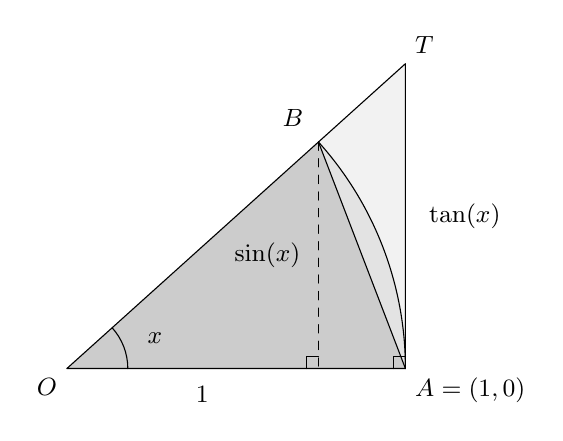
\begin{tikzpicture}[scale=4.3, line cap=round, line join=round,
                    every node/.style={font=\small}]
\coordinate (O) at (0,0);
\coordinate (A) at (1,0);
\coordinate (B) at ({cos(42)},{sin(42)});
\coordinate (T) at (1,{tan(42)});
\coordinate (H) at ({cos(42)},0);
\fill[gray!10] (O)--(A)--(T)--cycle;
\fill[gray!22] (O)--(A) arc[start angle=0,end angle=42,radius=1]--cycle;
\fill[gray!40] (O)--(A)--(B)--cycle;
\draw (O)--(A)--(T)--cycle;
\draw (A) arc[start angle=0,end angle=42,radius=1];
\draw (A)--(B);
\draw[dashed] (B)--(H) node[midway,left=3pt] {$\sin(x)$};
\draw (0.18,0) arc[start angle=0,end angle=42,radius=0.18];
\node at (0.26,0.09) {$x$};
\draw ({cos(42)-0.035},0)--({cos(42)-0.035},0.035)
      --({cos(42)},0.035);
\draw (0.965,0)--(0.965,0.035)--(1,0.035);
\node[below left] at (O) {$O$};
\node[below right] at (A) {$A=(1,0)$};
\node[above left=2pt] at (B) {$B$};
\node[above right] at (T) {$T$};
\node[right=5pt] at (1,{tan(42)/2}) {$\tan(x)$};
\node[below=3pt] at (0.4,0) {$1$};
\end{tikzpicture}
\end{center}

Both triangles have base $OA=1$, and their heights are $\sin(x)$ and
$\tan(x)$. The sector takes up the fraction $x/(2\pi)$ of a unit disk,
so its area is $(x/(2\pi))\pi=x/2$. Therefore
$$\frac{\sin(x)}2<\frac{x}2<\frac{\tan(x)}2,
\qquad\text{or}\qquad \sin(x)<x<\tan(x).$$

Before squeezing the quotient, we need $\cos(x)\to1$.
The first inequality and $\sin(-x)=-\sin(x)$ give
$|\sin(x)|\leq |x|$ near 0. Now use the trig identity
$1-\cos(x)=2\sin^2(x/2)$:
$$0\leq1-\cos(x)\leq2\left(\frac{|x|}{2}\right)^2
=\frac{x^2}{2}.$$
The right side tends to zero, so $\cos(x)\to1$.

Go back to the area inequalities. Dividing $\sin(x)<x$ by $x>0$
gives $\sin(x)/x<1$. Since $\tan(x)=\sin(x)/\cos(x)$ and $\cos(x)>0$,
the other inequality, $x<\tan(x)$, gives
$$\cos(x)<\frac{\sin(x)}x.$$
We have found our two bounds:
$$\cos(x)<\frac{\sin(x)}x<1.$$
Both approach 1, so the Squeeze Theorem gives the right-sided limit 1.
For a negative input write $x=-u$, where $u>0$. Then
$\sin(-u)/(-u)=\sin(u)/u$, so the left-sided limit is the same. Thus
\[
\lim_{x\to0}\frac{\sin(x)}x=1.
\qedhere
\]
\end{proof}

\proofheading{\texorpdfstring{$\displaystyle\lim_{x\to0}\frac{\cos(x)-1}{x}=0$}{lim x -> 0 (cos(x)-1)/x = 0}}{proof:cosine-limit}

\begin{proof}
We already know a sine quotient limit, so let's rewrite this quotient
to use it. The identity $\cos(x)-1=-2\sin^2(x/2)$ gives, for $x\ne0$,
\begin{align*}
\frac{\cos(x)-1}{x}
&=\frac{-2\sin^2(x/2)}{x}\\
&=-\sin(x/2)\frac{\sin(x/2)}{x/2}.
\end{align*}
As $x\to0$, the first sine factor tends to zero
(use $|\sin(x/2)|\leq |x|/2$ from the preceding proof).
The quotient tends to 1 by the sine limit, since its angle $x/2$
also tends to zero. The Product Law now gives
\[
\lim_{x\to0}\frac{\cos(x)-1}{x}=-(0)(1)=0.
\qedhere
\]
\end{proof}

\proofheading{\texorpdfstring{$\displaystyle\lim_{x\to\infty}\left(1+\frac1x\right)^x=e$}{lim x -> infinity (1+1/x)^x = e}}{proof:euler-limit}

\begin{proof}
Start with positive integer inputs. The
\hyperref[source:proof:binomial-theorem]{Binomial Theorem} gives
\begin{align*}
a_n=\left(1+\frac1n\right)^n
&=\sum_{k=0}^n\binom nk\frac1{n^k}\\
&=2+\sum_{k=2}^n\frac1{k!}
 \left(1-\frac1n\right)\left(1-\frac2n\right)
 \cdots\left(1-\frac{k-1}{n}\right).
\end{align*}
Notice that increasing $n$ makes each
factor in the last sum larger and adds another positive term.
So $a_n$ increases. Each factor is at most 1, and
$k!\geq2^{k-1}$, since $2,3,\ldots,k$ are all at least 2. Thus
$$2\leq a_n\leq2+\sum_{k=2}^n\frac1{2^{k-1}}
=3-\frac1{2^{n-1}}<3.$$
The \hyperref[sec:bounded-monotone-limits]{Bounded Monotone Limits}
result now tells us that $a_n$ has a limit. This is the
\hyperref[def:eulers-number]{number $e$} defined earlier.

For real inputs, choose $n$ with $n\leq x<n+1$. Since
$1+1/(n+1)\leq1+1/x\leq1+1/n$, comparing bases and exponents gives
$$
\frac{a_{n+1}}{1+1/(n+1)}
\leq\left(1+\frac1x\right)^x
\leq a_n\left(1+\frac1n\right).
$$
Both bounds approach $e$ as $x\to\infty$, so the Squeeze Theorem
gives the limit for real inputs too.

We'll also need the limit as $x\to-\infty$. Set $t=-x-1$, so
$t\to\infty$. Then
$$\left(1+\frac1x\right)^x
=\left(\frac{t}{t+1}\right)^{-(t+1)}
=\left(1+\frac1t\right)^t\left(1+\frac1t\right)
\longrightarrow e\cdot1=e.$$
\end{proof}

\proofheading{\texorpdfstring{$\displaystyle\lim_{x\to0}\frac{a^x-1}{x}=\ln(a)\quad(a>0)$}{lim x -> 0 (a^x-1)/x = ln(a), a > 0}}{proof:exponential-limit}

\begin{proof}
First we will find the limit for base $e$. We need an inequality that
compares $e^t$ with $1+t$, and we can get it using just multiplication.

For $u>-1$ and a positive integer $n$, we claim
$$(1+u)^n\geq1+nu.$$
For $n=1$ this is equality. If it is true for $n$, multiplying both
sides by the positive number $1+u$ gives
\begin{align*}
(1+u)^{n+1}
&\geq(1+nu)(1+u)\\
&=1+(n+1)u+nu^2\\
&\geq1+(n+1)u.
\end{align*}
The last step uses $nu^2\geq0$. So knowing the claim for one integer
proves it for the next. Starting at 1 proves it for every positive integer.
This is often called \textbf{Bernoulli's inequality}.

Fix any real number $t$. For sufficiently large $n$, we have $t/n>-1$,
so putting $u=t/n$ in the inequality gives
$$\left(1+\frac tn\right)^n\geq1+t.$$
If $t\ne0$, set $x=n/t$. Then
$$
\left(1+\frac tn\right)^n
=\left[\left(1+\frac1x\right)^x\right]^t\longrightarrow e^t.
$$
For $t>0$, $x\to\infty$; for $t<0$, $x\to-\infty$.
Both cases were proved above. Taking the fixed power $t$ is justified
by the Power Law, whose proof used continuity, not derivatives.
If $t=0$, the expression is always 1. We conclude that
$$e^t\geq1+t\qquad\text{for every real }t.$$

Now take $h>0$. Using $t=h$ gives $e^h-1\geq h$.
Using $t=-h$ gives an upper bound after a little rearranging:
$$e^{-h}\geq1-h
\quad\Longrightarrow\quad
1\geq e^h(1-h)
\quad\Longrightarrow\quad
e^h-1\leq he^h.$$
We multiplied by $e^h>0$, so the inequality kept its direction.
Divide the two bounds by $h>0$:
$$1\leq\frac{e^h-1}{h}\leq e^h.$$
Continuity of the exponential function gives $e^h\to1$, so the
Squeeze Theorem gives the right-sided limit 1. For the left side,
write $h=-k$ with $k>0$:
$$
\frac{e^h-1}{h}
=\frac{e^{-k}-1}{-k}
=e^{-k}\frac{e^k-1}{k}\longrightarrow(1)(1)=1.
$$
Thus $\lim_{h\to0}(e^h-1)/h=1$ from both sides.

Let's also record a logarithm limit for the Power Rule below.
Set $h=\ln(1+u)$, with $u>-1$ and $u\ne0$. Then $e^h-1=u$ and,
by logarithm continuity, $h\to0$ as $u\to0$. Therefore
$$
\frac{\ln(1+u)}u
=\frac{h}{e^h-1}
=\frac1{(e^h-1)/h}\longrightarrow1.
$$
We have used a reciprocal of the known quotient limit; we have not
assigned a value to a quotient with zero denominator.

Finally, change the base. For $a>0$, $a\ne1$, we have
$a^x=e^{x\ln(a)}$ and $\ln(a)\ne0$, so
$$
\frac{a^x-1}{x}
=\ln(a)\frac{e^{x\ln(a)}-1}{x\ln(a)}
\longrightarrow\ln(a).
$$
Here $x\ln(a)\to0$, so the fraction on the right has the base-$e$
limit just proved. If $a=1$, the original quotient is zero for every
$x\ne0$, which also gives $\ln(1)=0$.
\end{proof}



\proofchapter{Proofs from Chapter \ref*{sec:the-derivative}: The Derivative}
\label{sec:derivative-proofs}

\proofheading{Differentiability Implies Continuity (Theorem~\ref*{source:proof:differentiability-continuity})}{proof:differentiability-continuity}

\begin{proof}
Remember that differentiability at $a$ means
$$\frac{f(a+h)-f(a)}h\longrightarrow f'(a),$$
where $f'(a)$ is a finite number. To prove continuity, we instead need
the change $f(a+h)-f(a)$ itself to approach zero.

For $h\ne0$, multiply the difference quotient by $h$:
$$
f(a+h)-f(a)
=h\frac{f(a+h)-f(a)}h\longrightarrow(0)f'(a)=0.
$$
Thus $f(a+h)\to f(a)$, which says exactly that $f$ is continuous at $a$.
\end{proof}

\proofheading{The Product Rule}{proof:product-rule}
\label{sec:product-rule-proof}

\begin{proof}
Suppose $f$ and $g$ are differentiable at $a$. Start with the difference
quotient for their product. We want to separate it into the difference
quotients for $f$ and $g$. Adding and subtracting the same middle term,
$f(a+h)g(a)$, does this without changing the numerator:
\begin{align*}
&\frac{f(a+h)g(a+h)-f(a)g(a)}h\\
&\quad=\frac{f(a+h)g(a+h)-f(a+h)g(a)
       +f(a+h)g(a)-f(a)g(a)}h\\
&\quad=\frac{f(a+h)g(a+h)-f(a+h)g(a)}h
       +\frac{f(a+h)g(a)-f(a)g(a)}h\\
&\quad=\frac{f(a+h)\bigl(g(a+h)-g(a)\bigr)}h
       +\frac{g(a)\bigl(f(a+h)-f(a)\bigr)}h\\
&\quad=f(a+h)\frac{g(a+h)-g(a)}h
       +g(a)\frac{f(a+h)-f(a)}h.
\end{align*}
Since $f$ is differentiable, it is continuous, so $f(a+h)\to f(a)$.
The two difference quotients approach $g'(a)$ and $f'(a)$.
Taking the limit of the last line gives
\[
[fg]'(a)=f(a)g'(a)+g(a)f'(a).
\qedhere
\]
\end{proof}

\proofheading{The Chain Rule}{proof:chain-rule}
\label{sec:chain-rule-proof}

\begin{proof}
The idea is to separate the change in the outer function from the
change in the inner function. Suppose $g$ is differentiable at $a$ and
$f$ is differentiable at $b=g(a)$.

For a small change $k$ in the input to $f$, its difference quotient
is $(f(b+k)-f(b))/k$. There is a small snag: a change in $x$ can leave
$g(x)$ unchanged, so we must allow $k=0$ too. Define
$$
Q(k)=
\begin{cases}
\dfrac{f(b+k)-f(b)}k,&k\ne0,\\[6pt]
f'(b),&k=0.
\end{cases}
$$
This just fills the hole in the difference quotient with its limit.
The definition of the derivative says $Q(k)\to f'(b)=Q(0)$, so $Q$
is continuous at 0. We assigned $Q(0)$ separately; we did not divide by zero.
For every permitted $k$, including zero, we now have
$$f(b+k)-f(b)=Q(k)k.$$

When $x$ changes from $a$ to $a+h$, the change in the inner function is
$$k(h)=g(a+h)-g(a).$$
Differentiability of $g$ implies continuity, so $k(h)\to0$ as $h\to0$.
Substitute this inner change into the last identity and divide by $h\ne0$:
\begin{align*}
\frac{f(g(a+h))-f(g(a))}h
&=\frac{f(b+k(h))-f(b)}h\\
&=Q(k(h))\frac{k(h)}h.
\end{align*}
Even if $k(h)=0$, both sides are zero, so no input has been lost.
By continuity, $Q(k(h))\to f'(b)$. Also,
$$\frac{k(h)}h=\frac{g(a+h)-g(a)}h\longrightarrow g'(a).$$
The Product Law now gives
\[
[f\circ g]'(a)=f'(g(a))g'(a).
\qedhere
\]
\end{proof}

\proofheading{The Power Rule}{proof:power-rule}
\label{sec:power-rule-proof}

\begin{proof}
We will use $x^r=e^{r\ln(x)}$ for positive inputs. First, let's check
the exponential and logarithm derivatives we need, directly from the
special limits above. This keeps the argument from using the Power Rule
to prove itself.

For the exponential function, factor out $e^x$:
$$
\frac{e^{x+h}-e^x}h
=e^x\frac{e^h-1}h\longrightarrow e^x.
$$
So $[e^x]'=e^x$. For the logarithm, fix $x>0$ and take $h$ small
enough that $x+h>0$. The properties of logarithms give
\begin{align*}
\frac{\ln(x+h)-\ln(x)}h
&=\frac{\ln((x+h)/x)}h\\
&=\frac1x\frac{\ln(1+h/x)}{h/x}\longrightarrow\frac1x.
\end{align*}
The last fraction approaches 1 by the logarithm limit, with $h/x\to0$.
Thus $[\ln(x)]'=1/x$.

Now take any real $r$ and $x>0$. Apply the Chain Rule and the
Constant Multiple Rule:
\begin{align*}
[x^r]'
&=[e^{r\ln(x)}]'\\
&=e^{r\ln(x)}[r\ln(x)]'\\
&=x^r\frac rx\\
&=rx^{r-1}.
\end{align*}

For a negative input, a real power exists when $r=m/n$ is rational in
lowest terms with $n$ odd. This includes integers, where $n=1$.
Since $-x>0$, we can use the positive-input result on
$$x^r=(-1)^m(-x)^r.$$
The factor $(-1)^m$ is a constant, and $[-x]'=-1$, so
\begin{align*}
[x^r]'
&=-(-1)^m r(-x)^{r-1}\\
&=r\,\frac{(-1)^m(-x)^r}{x}\\
&=r\,\frac{x^r}{x}=rx^{r-1}.
\end{align*}
Other real exponents do not give real-valued powers at negative inputs.

At zero, we must check the definition instead of substituting into a
formula that might be undefined. If $r>0$ and the power is defined on
both sides of zero, its difference quotient is
$$\frac{h^r-0^r}h=\frac{h^r}h.$$
For $r>1$, its absolute value is $|h|^{r-1}\to0$, so the derivative is 0.
For $r=1$, the quotient is 1. For $0<r<1$, its absolute value is
$1/|h|^{1-r}$, which becomes unbounded, so there is no finite derivative.

Negative powers are undefined at zero. The constant function 1 has
derivative 0 wherever it is defined; if it is defined at zero as well,
its derivative there is still 0, without using the undefined expression
$0^0$. If a power is defined only for nonnegative inputs, the calculation
at zero is one-sided rather than a two-sided derivative.
\end{proof}

\proofheading{Derivatives of Even and Odd Functions (Theorem~\ref*{source:proof:even-odd-derivatives})}{proof:even-odd-derivatives}

\begin{proof}
The key is that replacing $x$ by $-x$ contributes a factor of $-1$
when we differentiate. The Chain Rule says
$$[f(-x)]'=f'(-x)[-x]'=-f'(-x).$$

If $f$ is even, then $f(-x)=f(x)$. Differentiate both sides:
$$-f'(-x)=f'(x),\qquad\text{so}\qquad f'(-x)=-f'(x).$$
That is exactly the definition of $f'$ being odd.

If $f$ is odd, start instead with $f(-x)=-f(x)$. Differentiation gives
$$-f'(-x)=-f'(x),\qquad\text{so}\qquad f'(-x)=f'(x).$$
That is exactly the definition of $f'$ being even.
These statements use the symmetric interval and differentiability
assumed in the theorem.
\end{proof}

\proofheading{An Even Function at the Origin (Theorem~\ref*{source:proof:even-derivative-zero})}{proof:even-derivative-zero}

\begin{proof}
An even graph is symmetric about the vertical axis. At the origin,
the difference quotients from opposite sides must therefore be opposites.
For $h\ne0$ sufficiently close to zero, $f(-h)=f(h)$, so
$$\frac{f(-h)-f(0)}{-h}
=-\frac{f(h)-f(0)}h.$$
As $h\to0$, the left side approaches $f'(0)$: its input change is $-h$,
which also tends to zero. The right side approaches $-f'(0)$.
Because the derivative exists, these must be the same finite number.
Thus $f'(0)=-f'(0)$, giving $2f'(0)=0$ and finally $f'(0)=0$.
\end{proof}

\proofchapter{Proofs from Chapter \ref*{sec:applications-of-derivatives}: Applications of Derivatives}
\label{sec:derivative-applications-proofs}

\proofheading{The Extreme Value Theorem (Theorem~\ref*{source:proof:extreme-value})}{proof:extreme-value}

\begin{proof}
We need to show two things: the heights of the graph stay bounded, and
the graph actually reaches its highest and lowest heights. If $a=b$,
there's only one height to consider, so suppose $a<b$.

First suppose the absolute values $|f(x)|$ weren't bounded. Cut $[a,b]$
into two closed halves. At least one half must still have unbounded
$|f(x)|$: if both had bounds, the larger bound would work for the whole
interval. Keep an unbounded half, cut it in half again, and keep going.

The \hyperref[sec:nested-interval-theorem]{Nested Interval Theorem} gives a
point $c$ in every retained interval. Since the lengths keep halving,
every point in a late enough interval is as close to $c$ as we like.
But continuity says that, near $c$, the heights stay close to the finite
number $f(c)$. In particular, we can make
$$|f(t)-f(c)|<1,$$
so that
$$|f(t)|\leq |f(c)|+|f(t)-f(c)|<|f(c)|+1.$$
This bounds all the heights on a late enough retained interval,
contradicting our choice of that interval. This argument also works when
$c$ is an endpoint, using continuity from inside $[a,b]$.

Now the heights are bounded. Let $M$ be their least upper bound, as in
\hyperref[sec:least-upper-bounds]{Least Upper Bounds}. All heights are at
most $M$, and some come as close to $M$ as we like. We still need to find
a point whose height is exactly $M$.

Again cut the interval in half. At least one half has heights coming
arbitrarily close to $M$. Otherwise each half would have an upper bound
smaller than $M$, and the larger of those two bounds would contradict
the choice of $M$. Keep a half whose heights approach $M$, and repeat.
The nested intervals give a common point $c$.

We know $f(c)\leq M$. Suppose $f(c)<M$, and put
$$T=\frac{f(c)+M}{2}.$$
Notice that $f(c)<T<M$. Continuity keeps all nearby heights below $T$.
Eventually a retained interval lies entirely that close to $c$, so all
its heights are below $T$. But that interval was chosen to have heights
arbitrarily close to $M$, including heights above $T$. This contradiction
shows that $f(c)=M$.

Finally, apply the same argument to the continuous function $-f$.
Wherever $-f$ reaches its maximum, $f$ reaches its minimum.
\end{proof}

\proofheading{Fermat's Theorem (Theorem~\ref*{source:proof:critical-numbers})}{proof:critical-numbers}

\begin{proof}
At a local maximum, nearby heights can't be greater than $f(a)$. Thus,
for small positive or negative $h$,
$$f(a+h)-f(a)\leq0.$$
Divide by $h$. On the right of $a$, $h>0$, so
$$\frac{f(a+h)-f(a)}h\leq0.$$
On the left, $h<0$, so dividing reverses the inequality:
$$\frac{f(a+h)-f(a)}h\geq0.$$
If $f'(a)$ exists, these two difference quotients must approach the
same number. The right-hand limit is at most 0 and the left-hand limit
is at least 0, so their common value must be 0. Thus $f'(a)=0$.

At a local minimum, $f(a+h)-f(a)\geq0$. The right-hand quotient is now
nonnegative and the left-hand quotient is nonpositive. Their common
limit is again 0.
\end{proof}

\proofheading{The Mean Value Theorem (Theorem~\ref*{source:proof:mean-value})}{proof:mean-value}

\begin{proof}
The goal is to find a tangent line with the same slope as the line
joining the endpoints. Call that slope
$$m=\frac{f(b)-f(a)}{b-a}.$$
The line joining the endpoints has equation $y=f(a)+m(x-a)$. Subtract
its height from the height of the graph:
$$F(x)=f(x)-f(a)-m(x-a).$$
This measures how far above or below that line the graph is. In
particular,
\begin{align*}
F(a)&=f(a)-f(a)-m(a-a)=0,\\
F(b)&=f(b)-f(a)-m(b-a)=0.
\end{align*}
The new function is still continuous on $[a,b]$ and differentiable
inside it.

If $F$ is zero at every input, its derivative is 0 at every interior point.
Otherwise $F$ has a positive value or a negative value somewhere. By
the Extreme Value Theorem, it reaches a positive maximum or a negative
minimum. That extremum can't be at an endpoint, since both endpoint
values are 0. So it occurs at an interior point $c$, where Fermat's
Theorem gives $F'(c)=0$.

Either way, there's an interior point $c$ with
\begin{align*}
0=F'(c)&=f'(c)-m,\\
f'(c)&=m=\frac{f(b)-f(a)}{b-a}.
\end{align*}
That's the tangent slope we wanted. Notice the special case: if a
function has equal endpoint heights, its derivative is 0 somewhere
between them. This is called \textbf{Rolle's theorem}.
\end{proof}

\proofheading{First Derivative Test (Theorem~\ref*{source:proof:first-derivative-test})}{proof:first-derivative-test}

\begin{proof}
We want to compare $f(a)$ with the heights just to its left and right.
Since $f$ is continuous at $a$ and differentiable on each side nearby,
the Mean Value Theorem applies between $a$ and any nearby $x\ne a$.
It gives a point $c$ between them with
$$\frac{f(x)-f(a)}{x-a}=f'(c),$$
or, multiplying by $x-a$,
$$f(x)-f(a)=f'(c)(x-a).$$
Now we only need to check the signs of the two factors.

Suppose $f'>0$ to the left of $a$ and $f'<0$ to the right. For $x<a$,
the point $c$ is also to the left, so $f'(c)>0$ while $x-a<0$. For
$x>a$, we have $f'(c)<0$ while $x-a>0$. The product is negative on
both sides, so $f(x)<f(a)$ on both sides. That's a local maximum.

If $f'<0$ on the left and $f'>0$ on the right, both products are
positive instead. Then $f(x)>f(a)$ on both sides, giving a local minimum.

If $f'>0$ on both sides, the product is negative on the left and
positive on the right. Thus there are nearby heights below and above
$f(a)$, so $f(a)$ is neither a local maximum nor a local minimum.
If $f'<0$ on both sides, the heights are above $f(a)$ on the left and
below it on the right, with the same conclusion.
\end{proof}

\proofheading{Second Derivative Test (Theorem~\ref*{source:proof:second-derivative-test})}{proof:second-derivative-test}

\begin{proof}
The idea is to use $f''$ to find the sign of $f'$, then use the First
Derivative Test. Suppose $f'(a)=0$ and $f''(a)>0$. Since $f''$ is
continuous at $a$, it stays positive close to $a$.

Apply the Mean Value Theorem to $f'$ between $a$ and a nearby $x$.
This is allowed because $f'$ is differentiable, and hence continuous,
there. For some $c$ between $a$ and $x$,
\begin{align*}
f'(x)-f'(a)&=f''(c)(x-a),\\
f'(x)&=f''(c)(x-a), &&\text{since $f'(a)=0$.}
\end{align*}
The factor $f''(c)$ is positive. Therefore $f'(x)<0$ when $x<a$ and
$f'(x)>0$ when $x>a$. The First Derivative Test gives a local minimum
at $a$. The needed continuity of $f$ at $a$ follows from differentiability
there.

If $f''(a)<0$, continuity keeps $f''(c)$ negative instead. The same
equation gives $f'(x)>0$ on the left and $f'(x)<0$ on the right, so the
First Derivative Test gives a local maximum.
\end{proof}

\proofheading{L'H\^opital's Rule (Theorem~\ref*{source:proof:lhopital})}{proof:lhopital}
\label{sec:lhopital-proof}

\begin{proof}
The main idea is a version of the Mean Value Theorem that compares two
functions. We'll prove that first, then use it for $0/0$ and
$\infty/\infty$. Throughout, we assume the hypotheses in the statement,
including $g\ne0$, $g'\ne0$, and
$$\frac{f'(x)}{g'(x)}\longrightarrow L.$$
The number $L$ is allowed to be $\infty$ or $-\infty$.

Suppose $f$ and $g$ are continuous on $[u,v]$ and differentiable inside
it, with $g'\ne0$. First, $g(v)\ne g(u)$: otherwise Rolle's theorem would
give a point where $g'=0$. So we can form the quotient of their changes,
$$A=\frac{f(v)-f(u)}{g(v)-g(u)}.$$
We want to relate this number to the derivatives. As in the Mean Value
Theorem proof, subtract a function that makes both endpoint heights 0.
This time we use a multiple of $g$:
$$H(t)=f(t)-f(u)-A\bigl(g(t)-g(u)\bigr).$$
At $t=u$, both differences are 0. At $t=v$, our choice of $A$ gives
$$H(v)=f(v)-f(u)-\frac{f(v)-f(u)}{g(v)-g(u)}
                     \bigl(g(v)-g(u)\bigr)=0.$$
Thus $H(u)=H(v)=0$. Rolle's theorem gives some $c\in(u,v)$ with
\begin{align*}
0=H'(c)&=f'(c)-Ag'(c),\\
Ag'(c)&=f'(c),\\
A&=\frac{f'(c)}{g'(c)}. &&\text{Here $g'(c)\ne0$.}
\end{align*}
In other words,
$$\frac{f(v)-f(u)}{g(v)-g(u)}=\frac{f'(c)}{g'(c)}.$$
This is the \textbf{Cauchy Mean Value Theorem}. Notice what it says:
the quotient of two changes equals the quotient of two derivatives at
some point between the inputs.

Now suppose we have $0/0$ as $x\to a^+$, where $a$ is finite. For this
argument, set $f(a)=g(a)=0$. Changing a value at the limiting input
doesn't change a limit, and these choices make both functions continuous
at $a$. Applying the result we just proved on $[a,x]$ gives
$$\frac{f(x)}{g(x)}
  =\frac{f(x)-f(a)}{g(x)-g(a)}
  =\frac{f'(c)}{g'(c)},\qquad a<c<x.$$
As $x$ approaches $a$ from the right, the point $c$ is trapped between
$a$ and $x$, so it approaches $a$ from the right too. Therefore the last
quotient approaches $L$, just as we wanted. This works for finite $L$
and for either infinite limit. For a left-hand limit, apply the same
argument on $[x,a]$; the two minus signs in the quotient cancel.

Next suppose we have $\infty/\infty$, still approaching a finite $a$
from one side. Either sign of infinity is allowed. We can't assign
finite endpoint values this time. Instead, choose a fixed nearby input
$b$ on that side and compare changes from $b$. The idea is that the
fixed numbers $f(b)$ and $g(b)$ will become negligible compared with
the unbounded function values.

First let $L$ be finite. Choose any small accuracy $\varepsilon>0$.
Since $f'/g'\to L$, we can choose $b$ close enough to $a$ that
$$\left|\frac{f'(t)}{g'(t)}-L\right|<\varepsilon$$
for every $t$ between $b$ and $a$. Now take $x$ between $b$ and $a$.
The Cauchy Mean Value Theorem, on the interval with endpoints $b$ and
$x$, says
$$R(x)=\frac{f(x)-f(b)}{g(x)-g(b)}=\frac{f'(c)}{g'(c)}$$
for some $c$ between $b$ and $x$. This point is also between $b$ and $a$,
so $|R(x)-L|<\varepsilon$.

We know $R(x)$ is close to $L$. Let's see how it relates to $f(x)/g(x)$:
\begin{align*}
R(x)\bigl(g(x)-g(b)\bigr)&=f(x)-f(b),\\
f(x)&=R(x)\bigl(g(x)-g(b)\bigr)+f(b),\\
\frac{f(x)}{g(x)}&=R(x)\left(1-\frac{g(b)}{g(x)}\right)
                         +\frac{f(b)}{g(x)}.
\end{align*}
To compare this with $L$, write $R(x)=(R(x)-L)+L$ and subtract $L$:
$$\frac{f(x)}{g(x)}-L
 =\bigl(R(x)-L\bigr)\left(1-\frac{g(b)}{g(x)}\right)
  +\frac{f(b)-Lg(b)}{g(x)}.$$
Here $b$ is fixed, while $|g(x)|\to\infty$. Thus the factor
$1-g(b)/g(x)$ approaches 1, and the last fraction approaches 0.
Close enough to $a$, the factor $1-g(b)/g(x)$ has absolute value less
than 2 and the last fraction has absolute value less than $\varepsilon$.
Consequently,
$$\left|\frac{f(x)}{g(x)}-L\right|
 <2\varepsilon+\varepsilon=3\varepsilon.$$
Since $\varepsilon$ can be as small as we like, this proves
$f(x)/g(x)\to L$.

If $L=\infty$, the goal is to make $f(x)/g(x)$ larger than any chosen
number $M>0$. Choose $b$ close enough that $f'(t)/g'(t)>4M$ between
$b$ and $a$. The same argument gives $R(x)>4M$ and
$$\frac{f(x)}{g(x)}
 =R(x)\left(1-\frac{g(b)}{g(x)}\right)+\frac{f(b)}{g(x)}.$$
Close enough to $a$, the factor in parentheses is greater than $1/2$
and $|f(b)/g(x)|<M$. Therefore
$$\frac{f(x)}{g(x)}>4M\left(\frac12\right)-M=M.$$
We can do this for every $M>0$, so the limit is $\infty$. If
$L=-\infty$, apply this result to $-f$ and $g$. Their derivative
quotient approaches $\infty$, so $-f/g\to\infty$, or $f/g\to-\infty$.
These arguments work on either side of $a$. Whenever the two one-sided
limits agree, they also give the two-sided limit.

Finally, we still need limits as $x\to\infty$ or $x\to-\infty$.
Set $t=1/x$, so these become $t\to0^+$ or $t\to0^-$, respectively.
Define
$$F(t)=f(1/t),\qquad G(t)=g(1/t).$$
These functions have the same indeterminate form as the original
quotient. The Chain Rule gives
$$F'(t)=-\frac{f'(1/t)}{t^2},\qquad
  G'(t)=-\frac{g'(1/t)}{t^2}.$$
The common factor $-1/t^2$ cancels, so
$$\frac{F'(t)}{G'(t)}=\frac{f'(1/t)}{g'(1/t)}\longrightarrow L.$$
Also $G$ and $G'$ are nonzero near 0, as required. Apply the appropriate
one-sided result we already proved to get $F(t)/G(t)\to L$. Since
$F(t)/G(t)=f(x)/g(x)$ when $t=1/x$, this proves the result at infinity
too, for both indeterminate forms and finite or infinite $L$.
\end{proof}

\proofchapter{Proofs from Chapter \ref*{sec:definite-integral}: The Definite Integral}

\subsection*{Rectangle Sums and Signed Area}
\label{sec:rectangle-sum-tools}

The idea is to trap the signed area between rectangles that are too low
and rectangles that are too high. Let's make that idea precise.

Divide $[a,b]$ at finitely many points
$$a=x_0<x_1<\cdots<x_n=b.$$
This division is called a \textbf{partition}, and we will call it $P$.
On the $j$th small interval, write $m_j$ for the greatest lower bound of
$f$ and $M_j$ for its least upper bound. In other words, $m_j$ is the
highest number that is no greater than any of the heights there, and
$M_j$ is the lowest number that is no less than any of them. For a
continuous function these are just its minimum and maximum. For any
bounded function, the bounds exist by
\hyperref[sec:least-upper-bounds]{Least Upper Bounds}.

Multiply each height bound by the corresponding rectangle width:
$$L_P=\sum_{j=1}^n m_j(x_j-x_{j-1}),\qquad
U_P=\sum_{j=1}^n M_j(x_j-x_{j-1}).$$
These are the \textbf{lower sum} and \textbf{upper sum}. Heights below
zero give negative contributions, just as in signed area. Any sum made
by choosing an actual function height on each interval lies between
$L_P$ and $U_P$.

Adding a dividing point splits one rectangle into two narrower ones.
Their lower heights can be higher, but cannot be lower than the old
lower height. So the lower sum cannot decrease. Similarly, the upper
sum cannot increase. If we have two different divisions, insert all
of their dividing points into one division. This shows that every lower
sum is at most every upper sum.

Let $I$ be the least upper bound of all the lower sums. The preceding
comparison gives
$$L_P\leq I\leq U_P$$
for every division $P$. If we can make $U_P-L_P$ smaller than any positive
number, these bounds pin down just one value. That value is the
\textbf{Riemann integral}. This makes the chapter's signed-area idea
precise: the lower and upper rectangle approximations can agree as
closely as we want.

\proofheading{Continuous Functions Are Integrable (Theorem~\ref*{source:proof:continuous-integrability})}{proof:continuous-integrability}
\label{sec:continuous-integrability}

\begin{proof}
The Extreme Value Theorem tells us that a continuous $f$ is bounded
on $[a,b]$, so the rectangle sums above make sense. We will show that
their gap can be made as small as we want. Assume $a<b$; an interval
of length zero has integral zero.

Fix a small height tolerance $\eta>0$. Divide $[a,b]$ into two equal
halves, then four equal pieces, then eight, and keep going. Call one of
these small intervals \textit{bad} if two heights of $f$ on it differ
by at least $\eta$.

Suppose there are bad intervals at arbitrarily late stages. At least one
of the first two halves must contain bad intervals at arbitrarily late
stages: otherwise each half would stop having them after some stage,
and so would the whole interval. Keep a half that has this property,
divide it in half, and make the same choice again.

The retained intervals sit inside one another, and their lengths tend
to zero. By the
\hyperref[sec:nested-interval-theorem]{Nested Interval Theorem}, they
shrink to a common point $c$. Continuity at $c$ says that all heights
sufficiently close to $c$ are within $\eta/3$ of $f(c)$. Eventually an
entire retained interval is that close to $c$. Any two of its heights
then differ by less than $2\eta/3$, so it cannot contain a bad interval.
This contradicts the way we chose it. At an endpoint, we use the same
argument with one-sided continuity.

Therefore some finite stage has no bad intervals. On each piece the
maximum minus the minimum is less than $\eta$, so
$$
U_P-L_P
=\sum_j(M_j-m_j)(x_j-x_{j-1})
<\eta\sum_j(x_j-x_{j-1})=\eta(b-a).
$$
Given an area tolerance $\varepsilon>0$, choose
$\eta=\varepsilon/(b-a)$. The upper and lower sums then differ by less
than $\varepsilon$, which proves integrability.
\end{proof}

\proofheading{Convergence of Riemann Sums (Theorem~\ref*{source:proof:riemann-sums})}{proof:riemann-sums}

\begin{proof}
We know that some division makes the lower and upper rectangle sums
close. We need to show that \textit{any} sufficiently fine division
works, including the equal-width divisions used in the chapter.

Given $\varepsilon>0$, choose a division $P$ with
$U_P-L_P<\varepsilon/2$. Let $m$ be its number of interior dividing
points, and choose $B\geq0$ with $|f(x)|\leq B$ on $[a,b]$.

Now make another division $Q$, with every width at most $\Delta x$.
Most of its small intervals lie entirely within one interval of $P$.
On each of these, the maximum possible height gap is no greater than
the gap on the containing interval of $P$. Their total contribution
to $U_Q-L_Q$ is therefore at most $U_P-L_P$.

The only exceptions are intervals of $Q$ that cross an interior dividing
point of $P$. There are at most $m$ of these: each contains at least
one of the $m$ dividing points, and different intervals cannot contain
the same point in their interiors. Each exceptional interval has width
at most $\Delta x$ and height gap at most $2B$, since its heights are
between $-B$ and $B$. Thus
$$U_Q-L_Q\leq U_P-L_P+2Bm\Delta x.$$
The numbers $B$ and $m$ are fixed. Make $\Delta x$ small enough that
$2Bm\Delta x<\varepsilon/2$; if $Bm=0$, that term is already zero.
Then $U_Q-L_Q<\varepsilon$.

Choose any one function height on each interval of $Q$ and add the
resulting rectangle areas. This sum and the integral both lie between
$L_Q$ and $U_Q$, so they differ by less than $\varepsilon$. This proves
convergence as the largest width tends to zero. Left and right endpoint
sums are two such choices. Finally, the trapezoid sum is
$T_n=(L_n+R_n)/2$, so it has the same limit.
\end{proof}

\proofheading{Polynomial Sum Identities}{proof:polynomial-sums}

\begin{proof}
Let $n$ be a positive integer. The constant sum $\sum_{k=1}^n1=n$
just counts $n$ copies of 1.

For the other identities, write $S_j=\sum_{k=1}^n k^j$.
To find $S_1$, write the same sum forwards and backwards:
\begin{align*}
S_1&=1+2+\cdots+n,\\
S_1&=n+(n-1)+\cdots+1.
\end{align*}
Adding gives $n$ copies of $n+1$, so
$$2S_1=n(n+1),\qquad S_1=\frac{n(n+1)}2.$$

For the squares, expand $(k+1)^3-k^3=3k^2+3k+1$ and sum from
$k=1$ to $n$. On the left, every interior cube cancels:
$$(n+1)^3-1=3S_2+3S_1+n.$$
Substitute the formula for $S_1$ and rearrange:
\begin{align*}
3S_2&=(n+1)^3-1-\frac{3n(n+1)}2-n\\
&=n^3+3n^2+3n-\frac{3n^2+3n}{2}-n\\
&=n^3+\frac32n^2+\frac12n\\
&=\frac{n(2n^2+3n+1)}2\\
&=\frac{n(n+1)(2n+1)}2.
\end{align*}
Thus $S_2=n(n+1)(2n+1)/6$.

For the cubes, expand $(k+1)^4-k^4=4k^3+6k^2+4k+1$.
Summing and canceling the interior fourth powers gives
$$(n+1)^4-1=4S_3+6S_2+4S_1+n.$$
Using the two formulas just proved,
\begin{align*}
4S_3&=(n+1)^4-1-n(n+1)(2n+1)-2n(n+1)-n\\
&=(n^4+4n^3+6n^2+4n)\\
&\quad-(2n^3+3n^2+n)-(2n^2+2n)-n\\
&=n^4+2n^3+n^2\\
&=n^2(n+1)^2.
\end{align*}
Therefore $S_3=n^2(n+1)^2/4$.
\end{proof}

\proofheading{The Finite Geometric Sum}{proof:finite-geometric-sum}

\begin{proof}
Let $n$ be a positive integer and write the sum as $S$.
Multiplying by $r$ shifts every power up by one:
\begin{align*}
S&=r+r^2+\cdots+r^n,\\
rS&=r^2+r^3+\cdots+r^{n+1}.
\end{align*}
Subtract the second line from the first. All the middle terms cancel:
$$(1-r)S=r-r^{n+1}=r(1-r^n).$$
For $r\ne1$, divide by $1-r$ to get
$$\sum_{k=1}^n r^k=\frac{r(1-r^n)}{1-r}.$$
If $r=1$, there are $n$ copies of 1, so the sum is $n$.
\end{proof}

\subsection*{Algebra of Definite Integrals}

We will use a few integral rules below, so let's explain why they follow
from rectangles. Suppose $f$ and $g$ are integrable. Choose divisions
that make their upper-minus-lower gaps small, then insert all the dividing
points into one common division. Adding points cannot increase either
gap. On each small interval, the height gap for $f+g$ is at most the
height gap for $f$ plus the height gap for $g$. Therefore the total
upper-minus-lower gap for $f+g$ is at most the sum of those for $f$ and
$g$, and can be made as small as we want. Thus $f+g$ is integrable.

Multiplying heights by a constant $C$ multiplies the gap by $|C|$;
when $C<0$, the upper and lower heights trade places. So $Cf$ is also
integrable. On the same division, with the same chosen inputs, the
rectangle sum for $Cf+g$ is $C$ times the sum for $f$ plus the sum for
$g$. Taking limits proves
$$\int_a^b(Cf(x)+g(x))\,dx
=C\int_a^b f(x)\,dx+\int_a^b g(x)\,dx.$$

We can also put the rectangles on $[a,b]$ next to those on $[b,c]$.
Their sums add, giving
$$\int_a^b f(t)\,dt+\int_b^c f(t)\,dt=\int_a^c f(t)\,dt.$$
Reversing the bounds changes the sign by definition.

Finally, if $|g|\leq M$, every rectangle has absolute area at most
$M$ times its width. The absolute value of their sum is no greater than
the sum of those absolute areas. Taking limits gives
$$\left|\int_u^v g(t)\,dt\right|\leq M|v-u|.$$
A constant $C$ integrates to $C(v-u)$ because every rectangle sum is
already that number.

\proofheading{The Fundamental Theorem of Calculus (Theorem~\ref*{source:proof:fundamental-theorem})}{proof:fundamental-theorem}

\begin{proof}
Suppose $f$ is continuous on $[a,b]$, and set
$$A(x)=\int_a^x f(t)\,dt.$$
The idea in the first part is that adding a short interval adds an
amount of signed area close to its width times $f(x)$.

First, $|f|$ is bounded by some $M$ on $[a,b]$. Moving from $x$ to $y$
can change the accumulated area by at most $M|y-x|$, so
$$|A(y)-A(x)|\leq M|y-x|.$$
This tends to zero as $y\to x$, proving that $A$ is continuous, including
one-sided continuity at the endpoints.

For $a<x<b$ and a sufficiently small nonzero $h$, additivity gives
$$A(x+h)-A(x)=\int_x^{x+h}f(t)\,dt.$$
A constant height $f(x)$ has integral $hf(x)$ on the same interval.
Subtract it and divide by $h$:
$$
\frac{A(x+h)-A(x)}h-f(x)
=\frac1h\int_x^{x+h}\bigl(f(t)-f(x)\bigr)\,dt.
$$
By continuity, if $|h|$ is small enough, every $t$ between $x$ and $x+h$
satisfies $|f(t)-f(x)|<\varepsilon$. The integral on the right has
absolute value at most $\varepsilon|h|$. Therefore
$$
\left|\frac{A(x+h)-A(x)}h-f(x)\right|
\leq\frac{\varepsilon|h|}{|h|}=\varepsilon.
$$
This works for either sign of $h$, and proves $A'(x)=f(x)$.

For the second part, let $F$ be continuous on $[a,b]$ with $F'=f$
on $(a,b)$. Notice that $F$ and $A$ have the same derivative there, so
$$[F-A]'=f-f=0.$$
The Mean Value Theorem says that a function with zero derivative is
constant: its change between two inputs is its derivative at some
intermediate input times the distance between them, which is zero.
Thus $F(b)-A(b)=F(a)-A(a)$. Since $A(a)=0$, rearranging gives
$$\int_a^b f(x)\,dx=A(b)=F(b)-F(a).$$
\end{proof}

\proofchapter{Proofs from Chapter \ref*{sec:indefinite-integral}: The Indefinite Integral}

\proofheading{Integration by Parts}{proof:integration-by-parts}

\begin{proof}
Integration by parts comes from reading the Product Rule backwards.
Suppose $f$ and $g$ are differentiable on an interval. Let $H$ be an
antiderivative of $fg'$, so $H'=fg'$. We assume this antiderivative exists
when we write its indefinite integral.

Subtracting $H$ from the product leaves an antiderivative of $f'g$:
\begin{align*}
[fg-H]'&=f'g+fg'-H' &&\text{(Product and Difference Rules)}\\
&=f'g+fg'-fg' &&\text{(since $H'=fg'$)}\\
&=f'g. &&\text{(cancel)}
\end{align*}
Therefore
$$\int f'(x)g(x)\,dx=f(x)g(x)-H(x)+C.$$
Writing $H$ as $\int f(x)g'(x)\,dx$ gives the integration by parts
formula. Any choice of constant in $H$ is absorbed into $C$.

When the products $f'g$ and $fg'$ are continuous on $[a,b]$, the
Fundamental Theorem of Calculus gives the definite version:
$$\int_a^b f'(x)g(x)\,dx
=f(b)g(b)-f(a)g(a)-\int_a^b f(x)g'(x)\,dx.$$
\end{proof}

\proofheading{\texorpdfstring{$u$-Substitution}{u-Substitution}}{proof:u-substitution}

\begin{proof}
Substitution comes from reading the Chain Rule backwards. Suppose
$g$ is differentiable and $f$ is differentiable on an interval containing
the values of $g$. Then
$$[f(g(x))]'=f'(g(x))g'(x).$$
In other words, we already know an antiderivative of the expression on
the right:
$$\int f'(g(x))g'(x)\,dx=f(g(x))+C.$$
The substitution $u=g(x)$ gives the inner expression a shorter name,
and $du=g'(x)\,dx$ records its derivative. With those replacements the
same calculation becomes
$$\int f'(g(x))g'(x)\,dx=\int f'(u)\,du=f(u)+C.$$
Finally, replace $u$ by $g(x)$ to write the answer in the original variable.

If the derivatives are continuous, the Fundamental Theorem gives
$$\int_a^b f'(g(x))g'(x)\,dx=f(g(b))-f(g(a)).$$
Applying the same theorem in the $u$ variable shows that this equals
$$\int_{g(a)}^{g(b)}f'(u)\,du.$$
This explains why the bounds change from $a,b$ to $g(a),g(b)$. It also
works when the new lower bound is larger than the new upper bound,
because reversing integral bounds changes the sign.
\end{proof}

\proofchapter{Proofs from Chapter \ref*{sec:more-definite-integrals}: More Definite Integrals}

\proofheading{Comparison Theorem for Integrals (Theorem~\ref*{source:proof:integral-comparison})}{proof:integral-comparison}

\begin{proof}
On a closed interval where both functions are integrable, choose
the same rectangle widths and the same sample inputs for both. Since
$0\leq f(x)\leq g(x)$, each rectangle for $f$ has area no greater than
the corresponding rectangle for $g$. Adding and taking limits gives
$$0\leq\int_a^b f(x)\,dx\leq\int_a^b g(x)\,dx.$$

An improper integral is a limit of ordinary integrals, so apply this
inequality \textit{before} taking that limit. On $[a,\infty)$, for instance,
$$0\leq\int_a^t f(x)\,dx\leq\int_a^t g(x)\,dx.$$
Because both functions are nonnegative, increasing $t$ can only increase
these integrals. If the integral of $g$ converges to a finite number,
that number bounds all the integrals of $f$. They are increasing and
bounded, so they have a finite limit by
\hyperref[sec:bounded-monotone-limits]{Bounded Monotone Limits}.

On the other hand, if the integral of $f$ diverges, these nonnegative,
increasing integrals cannot stay bounded. They grow without bound,
forcing the larger integrals of $g$ to do the same.

At a finite improper endpoint, move the endpoint toward the singularity
instead of toward infinity; the same area comparison applies. At an
interior singularity, split the integral there and apply the comparison
to the two pieces separately.
\end{proof}

\proofheading{Additivity and Reversal of Integration Limits (Theorem~\ref*{source:proof:integral-additivity})}{proof:integral-additivity}

\begin{proof}
First suppose $a<b<c$. Divide $[a,b]$ and $[b,c]$ into small intervals,
and choose a rectangle height on each. Put the two lists of rectangles
together. They now cover $[a,c]$, and their total area is exactly the sum
of the two smaller totals. Let all the widths tend to zero:
$$\int_a^b f(x)\,dx+\int_b^c f(x)\,dx=\int_a^c f(x)\,dx.$$

Reversing the bounds means moving through the interval in the opposite
direction. We record this by defining
$$\int_b^a f(x)\,dx=-\int_a^b f(x)\,dx.$$
The splitting equation then works for any order of $a,b,c$. To see why,
first split at whichever of the three numbers lies in the middle, then
move an integral to the other side of the equation and reverse its
bounds when necessary. If two bounds agree, the integral between them
is zero, so the equation still holds.

For improper integrals, first do this on closed intervals away from any
singularity, and then take the required endpoint limits. The assumption
that the integrals are finite lets us add and subtract these limits;
it rules out expressions such as $\infty-\infty$.
\end{proof}

\proofchapter{Proofs from Chapter \ref*{sec:solving-odes}: Solving ODEs}

\proofheading{Euler's Formula (Theorem~\ref*{source:proof:eulers-formula})}{proof:eulers-formula}

\begin{proof}
We use the real exponential, sine, and cosine series from
Chapter~\ref{sec:power-series}. First, let's explain what the
exponential means for a complex input.
For $z=a+ib$, its absolute value $|z|=\sqrt{a^2+b^2}$ is its distance
from zero. Multiplying complex numbers gives $|zw|=|z||w|$, so
$|z^n|=|z|^n$. We say that complex numbers approach a limit when their
real parts and imaginary parts approach the corresponding real limits.

Define the complex exponential by
$$E(z)=\sum_{n=0}^{\infty}\frac{z^n}{n!}.$$
Why does this series have a sum? The absolute value of its $n$th term is
$|z|^n/n!$, and the real exponential series gives
$$\sum_{n=0}^{\infty}\left|\frac{z^n}{n!}\right|
=\sum_{n=0}^{\infty}\frac{|z|^n}{n!}=e^{|z|}<\infty.$$
Each term's real and imaginary parts have absolute values no greater
than that term's absolute value. The real Comparison and Absolute
Convergence Tests therefore make both component series converge.
Their two sums define $E(z)$.
For real $z$, this is exactly the known Maclaurin series for $e^z$.
Thus $E$ extends the usual exponential, and we write it as $e^z$ too.

Now let $v$ be real. The powers of $i$ cycle through $1,i,-1,-i$.
For the finite partial sums
$$P_N(z)=\sum_{n=0}^{N}\frac{z^n}{n!},$$
separating the even and odd powers gives the exact equality
$$
P_{2N+1}(iv)
=\sum_{k=0}^{N}\frac{(-1)^kv^{2k}}{(2k)!}
 +i\sum_{k=0}^{N}\frac{(-1)^kv^{2k+1}}{(2k+1)!}.
$$
The two sums on the right approach the real cosine and sine series.
Taking their limits proves
$$E(iv)=\cos(v)+i\sin(v).$$
We separated finite sums first, so no rearrangement of an infinite
series was needed.

To handle a general input $u+iv$, we still need the exponent rule
$E(w+z)=E(w)E(z)$. Let's prove it using finite multiplication.
Multiplying $P_N(w)$ and $P_N(z)$ gives terms
$$\frac{w^m z^n}{m!\,n!},\qquad 0\leq m,n\leq N.$$
Here the pair $(m,n)$ records which term we chose from each factor.
Keep the pairs with $m+n\leq N$, and collect those with the same
total $k=m+n$. Their sum is
\begin{align*}
\sum_{k=0}^{N}\sum_{m=0}^{k}
 \frac{w^m z^{k-m}}{m!\,(k-m)!}
&=\sum_{k=0}^{N}\frac1{k!}
 \sum_{m=0}^{k}{k\choose m}w^m z^{k-m}\\
&=\sum_{k=0}^{N}\frac{(w+z)^k}{k!}=P_N(w+z).
\end{align*}
The middle equality is just the finite binomial expansion.

What about the discarded pairs? They satisfy $m+n>N$, so at least
one of $m$ and $n$ is greater than $N/2$. The triangle inequality
bounds the absolute value of their sum by the sum of their absolute
values. For the pairs with $m>N/2$, add the $w$ terms after that index
and bound the sum of the $z$ terms by $e^{|z|}$.
Do the same with the roles reversed for $n>N/2$. Counting some pairs
twice only makes our upper bound larger. Therefore
\begin{align*}
|P_N(w)P_N(z)-P_N(w+z)|
&\leq e^{|z|}\sum_{m>N/2}\frac{|w|^m}{m!}\\
&\quad+e^{|w|}\sum_{n>N/2}\frac{|z|^n}{n!}
\longrightarrow0.
\end{align*}
Both sums on the right are what remains after removing more and more
initial terms from convergent real exponential series. Each remaining
sum tends to zero, because its initial partial sum approaches the full sum.
Limits of complex products follow from the real Limit Laws: multiply
the real and imaginary parts and take their limits separately.
Thus the left-hand product approaches $E(w)E(z)$, while
$P_N(w+z)\to E(w+z)$. Their difference tends to zero, proving
$$E(w+z)=E(w)E(z).$$

Finally, take $w=u$ and $z=iv$, with $u,v$ real. Using the real
exponential and the pure imaginary case already proved,
\[
e^{u+iv}=E(u)E(iv)=e^u\bigl(\cos(v)+i\sin(v)\bigr).
\qedhere
\]
\end{proof}

\proofheading{Superposition Principle (Theorem~\ref*{source:proof:homogeneous-solutions})}{proof:homogeneous-solutions}

\begin{proof}
For the equation $ay''+by'+cy=0$, suppose $y_1$ and $y_2$ are solutions
and $p,q$ are constants. Set $y=py_1+qy_2$. The Sum and Scalar Multiple
Rules give
$$
y'=py_1'+qy_2',\qquad y''=py_1''+qy_2''.
$$
Substitute these into the left side of the equation and group terms:
\begin{align*}
ay''+by'+cy
&=p(ay_1''+by_1'+cy_1)\\
&\quad+q(ay_2''+by_2'+cy_2)\\
&=p\cdot0+q\cdot0=0.
\end{align*}
Thus $y$ is another solution. Notice why the terms separate: each term
is a coefficient times $y$ or one of its derivatives, and the right side
of the equation is zero. This is what we need from \textit{linear and
homogeneous}. The same grouping works when the coefficients depend
on $x$ or when higher derivatives appear. A nonlinear term such as
$y^2$ would not separate this way.
\end{proof}

\proofchapter{Proofs from Chapter \ref*{sec:sequences}: Sequences}

\proofheading{Bounded Monotone Sequences (Theorem~\ref*{source:proof:monotone-sequences})}{proof:monotone-sequences}

\begin{proof}
Suppose $(a_n)$ is bounded and increasing. Here increasing allows
$a_{n+1}=a_n$. Let $S$ be the least upper bound of its terms, as in
\hyperref[sec:least-upper-bounds]{Least Upper Bounds}. We expect the
terms to approach $S$: they keep moving upward, but cannot pass it.

To check this, choose any $\varepsilon>0$. Some term must satisfy
$a_N>S-\varepsilon$. Otherwise $S-\varepsilon$ would already be an upper
bound, contradicting that $S$ is the \textit{least} upper bound. Because
the sequence is increasing, every later term satisfies
$$S-\varepsilon<a_N\leq a_n\leq S\qquad(n\geq N).$$
Thus $|a_n-S|<\varepsilon$ from that point onward, which is exactly what
$a_n\to S$ means.

If $(a_n)$ is decreasing and bounded, then $(-a_n)$ is increasing and
bounded. Apply the same argument and negate the resulting limit.
\end{proof}

\proofchapter{Proofs from Chapter \ref*{sec:series}: Series}

\proofheading{The Geometric Series}{proof:geometric-series}

\begin{proof}
Remember that a series converges when its finite partial sums approach
a finite number. For the geometric series, we can calculate those
partial sums. Write
$$S_N=1+r+\cdots+r^{N-1}.$$
Multiplying by $r$ shifts every power up one place. Subtracting cancels
the middle terms:
$$S_N-rS_N=1-r^N.$$
For $r\ne1$, this gives
$$S_N=\frac{1-r^N}{1-r}.$$

If $|r|<1$, then $r^N\to0$. For $0<|r|<1$, you can see this from
$|r|^N=e^{N\ln|r|}$: since $\ln|r|<0$, the exponent goes to $-\infty$.
The case $r=0$ is immediate. Taking the limit of $S_N$ now gives
$1/(1-r)$. Multiplying all terms by the first term gives the corresponding
formula for any geometric series, including
$$\sum_{n=k}^{\infty}r^n=\frac{r^k}{1-r}$$
whenever the displayed powers are defined and $|r|<1$.

If these partial sums converged, their consecutive differences would
approach zero. But $S_{N+1}-S_N=r^N$, whose magnitude is at least $1$
when $|r|\geq1$. So the geometric series with first term $1$ diverges
in that case, as does any nonzero constant multiple of it.
\end{proof}

\proofheading{Divergence Test (Theorem~\ref*{source:proof:divergence-test})}{proof:divergence-test}

\begin{proof}
Suppose $\sum a_n$ converges to $S$. Its $n$th partial sum is
$$S_n=a_1+a_2+\cdots+a_n.$$
Both $S_n$ and $S_{n-1}$ approach $S$: omitting one position in a
sequence does not change its limit. Subtracting the two sums leaves
just the newest term, so
$$a_n=S_n-S_{n-1}\longrightarrow S-S=0.$$
Therefore, if $a_n$ fails to approach zero, the series cannot converge.
This includes both a nonzero limit and no limit at all.
\end{proof}

\proofheading{Integral Test (Theorem~\ref*{source:proof:integral-test})}{proof:integral-test}

\begin{proof}
The idea is to put the decreasing graph between rectangles of width
$1$. Suppose $f$ is positive, continuous, and decreasing on
$[k,\infty)$, where $k$ is a positive integer, and $a_n=f(n)$.
For $n\leq x\leq n+1$, decreasing means
$$f(n+1)\leq f(x)\leq f(n).$$
The rectangle with the right endpoint height lies below the graph, and
the one with the left endpoint height lies above it. Their widths are
$1$, so
$$f(n+1)\leq\int_n^{n+1}f(x)\,dx\leq f(n).$$

Adding the upper estimates from $n=k$ through $N$, and the lower
estimates from $n=k$ through $N-1$, gives
$$
\int_k^{N+1}f(x)\,dx\leq\sum_{n=k}^N a_n
\leq a_k+\int_k^N f(x)\,dx.
$$
The extra $a_k$ on the right is the first rectangle, which is left over
when the lower-height rectangles start at $a_{k+1}$.

If the improper integral converges, the right side bounds all the
partial sums from above. The partial sums increase because $a_n>0$.
An increasing, bounded sequence converges, so the series converges.

Conversely, if the series converges, the left inequality bounds the
integrals at integer endpoints. It bounds all intervening endpoints too,
since adding area under a positive graph only increases the integral.
The integrals are therefore increasing and bounded. By
\hyperref[sec:bounded-monotone-limits]{Bounded Monotone Limits}, they
approach a finite number. That is exactly convergence of the improper
integral.
\end{proof}

\proofheading{The $p$-series Test (Theorem~\ref*{source:proof:p-series-test})}{proof:p-series-test}

\begin{proof}
For $p>0$, $f(x)=x^{-p}$ is positive, continuous, and decreasing for
$x>0$, so we can use the Integral Test. When $p\ne1$,
$$\int_k^t x^{-p}\,dx=\frac{t^{1-p}-k^{1-p}}{1-p}.$$
If $p>1$, then $1-p<0$ and $t^{1-p}\to0$, giving a finite limit. If
$0<p<1$, then $t^{1-p}\to\infty$ and $1-p>0$, so the integral grows
without bound. For $p=1$, it is
$$\int_k^t\frac1x\,dx=\ln(t)-\ln(k)\longrightarrow\infty.$$
The Integral Test gives the same convergence or divergence for the
corresponding series.

Finally, if $p\leq0$, the terms $1/n^p$ are at least $1$. They cannot
approach zero, so the Divergence Test makes the series diverge.
\end{proof}

\proofheading{Comparison Test (Theorem~\ref*{source:proof:series-comparison})}{proof:series-comparison}

\begin{proof}
Suppose $0\leq a_n\leq b_n$ and $\sum b_n$ converges to $B$.
Adding the term-by-term inequalities gives
$$0\leq\sum_{n=1}^N a_n\leq\sum_{n=1}^N b_n\leq B.$$
The partial sums on the left increase, because their terms are
nonnegative, and they never exceed $B$. The Bounded Monotone Sequences
Theorem therefore says they converge. This proves convergence of
$\sum a_n$.

The divergence conclusion is the same statement read backwards:
if $\sum a_n$ diverges, then $\sum b_n$ cannot converge, because its
convergence would force $\sum a_n$ to converge.

The comparison need only hold after some fixed index. Adding or removing
finitely many initial terms adds or subtracts a fixed number from every
later partial sum, so it does not change whether a finite limit exists.
\end{proof}

\proofheading{Limit Comparison Test (Theorem~\ref*{source:proof:limit-comparison})}{proof:limit-comparison}

\begin{proof}
Suppose $a_n\geq0$, $b_n>0$, and $a_n/b_n\to c$ with
$0<c<\infty$. The ratio approaching $c$ means that eventually it stays
within $c/2$ of $c$. From some index onward, therefore,
$$\frac c2<\frac{a_n}{b_n}<\frac{3c}{2}.$$
Multiplying by the positive $b_n$ gives ordinary comparisons:
$$\frac c2 b_n<a_n<\frac{3c}{2}b_n.$$

If $\sum b_n$ converges, so does its constant multiple
$\sum (3c/2)b_n$, and the upper bound makes $\sum a_n$ converge.
If $\sum a_n$ converges, rewrite the lower bound as
$b_n<(2/c)a_n$. Comparison now makes $\sum b_n$ converge.
Ignoring the finitely many terms before the inequalities hold does not
change convergence. Thus either both series converge or both diverge.
\end{proof}

\proofheading{Alternating Series Test (Theorem~\ref*{source:proof:alternating-test})}{proof:alternating-test}

\begin{proof}
Consider $b_1-b_2+b_3-b_4+\cdots$, where $b_n\geq0$ decreases to
zero. Write $S_N$ for its first $N$ terms. The idea is that each positive
term moves the sum upward and the next, smaller negative term moves it
back down. We will show that these two kinds of partial sum approach
the same number.

The even partial sums increase:
$$S_{2m+2}-S_{2m}=b_{2m+1}-b_{2m+2}\geq0.$$
The odd partial sums decrease:
$$S_{2m+3}-S_{2m+1}=-b_{2m+2}+b_{2m+3}\leq0.$$
We also have
$$0\leq S_{2m}\leq S_{2m+1}\leq b_1.$$
For the first inequality, group the even sum as
$(b_1-b_2)+\cdots+(b_{2m-1}-b_{2m})$; each pair is nonnegative.
For the last, write the odd sum as
$b_1-(b_2-b_3)-\cdots-(b_{2m}-b_{2m+1})$.
The middle inequality is $S_{2m+1}-S_{2m}=b_{2m+1}\geq0$.

Thus the even sums form a bounded increasing sequence, and the odd
sums form a bounded decreasing sequence. Both have limits by the
Bounded Monotone Sequences Theorem. Their limits agree because
$$S_{2m+1}-S_{2m}=b_{2m+1}\longrightarrow0.$$
Every partial sum is either even or odd, so all partial sums approach
this common limit. The series converges. Starting with a negative term
just multiplies every partial sum, and its limit, by $-1$.
\end{proof}

\proofheading{Absolute Convergence Test (Theorem~\ref*{source:proof:absolute-convergence})}{proof:absolute-convergence}

\begin{proof}
Suppose $\sum|a_n|$ converges. Separate each term into a nonnegative
part and the magnitude of its negative part. If $a_n\geq0$, set
$p_n=a_n$ and $q_n=0$. If $a_n<0$, set $p_n=0$ and $q_n=-a_n$.
In both cases,
$$a_n=p_n-q_n,\qquad 0\leq p_n\leq|a_n|,\qquad
0\leq q_n\leq|a_n|.$$
Comparison with $\sum|a_n|$ shows that $\sum p_n$ and $\sum q_n$
both converge, say to $P$ and $Q$.

For every finite partial sum,
$$\sum_{n=1}^N a_n=\sum_{n=1}^N p_n-\sum_{n=1}^N q_n.$$
Taking limits gives $P-Q$, a finite number. Thus $\sum a_n$ converges.
\end{proof}

\proofheading{Ratio Test (Theorem~\ref*{source:proof:ratio-test})}{proof:ratio-test}

\begin{proof}
Assume the terms are nonzero from some index onward, so the ratios
are defined. The idea is to compare successive magnitudes with those
of a geometric series.

Suppose $|a_{n+1}/a_n|\to L<1$. Choose a number $q$ strictly between
$L$ and $1$. Because the ratios approach $L$, there is an index $N$
after which
$$|a_{n+1}|\leq q|a_n|.$$
Apply this repeatedly:
$$|a_{N+1}|\leq q|a_N|,\qquad
|a_{N+2}|\leq q|a_{N+1}|\leq q^2|a_N|,$$
and, in general,
$$|a_{N+j}|\leq |a_N|q^j\qquad(j\geq0).$$
The numbers on the right have finite sum $|a_N|/(1-q)$, since $q<1$.
Comparison proves that the sum of the $|a_n|$ from $N$ onward converges.
Adding back the finitely many earlier terms proves absolute convergence.

If $L>1$, including $L=\infty$, choose $1<q<L$. Eventually the ratios
are greater than $q$, so repeating the inequality gives
$|a_{N+j}|\geq |a_N|q^j$. These magnitudes grow without bound, rather
than approach zero. The Divergence Test applies.

When $L=1$, these geometric comparisons do not decide convergence.
The series $\sum1/n$ diverges, $\sum(-1)^{n+1}/n$ converges
conditionally, and $\sum1/n^2$ converges absolutely, but their absolute
ratios all approach $1$. For instance, for terms of magnitude $1/n^p$
the ratio is $(n/(n+1))^p\to1$.
\end{proof}

\proofheading{Root Test (Theorem~\ref*{source:proof:root-test})}{proof:root-test}

\begin{proof}
Again we compare magnitudes with a geometric series. Suppose
$\sqrt[n]{|a_n|}\to L<1$. Choose $q$ with $L<q<1$. From some index
onward, $\sqrt[n]{|a_n|}\leq q$. Raising both nonnegative sides to
the $n$th power gives
$$|a_n|\leq q^n.$$
The geometric series $\sum q^n$ converges, so comparison proves that
$\sum|a_n|$ converges. Finitely many earlier terms do not affect this.

If $L>1$, including $L=\infty$, choose $1<q<L$. Eventually
$\sqrt[n]{|a_n|}\geq q$, giving $|a_n|\geq q^n$. The terms do not
approach zero, so the original series diverges.

At $L=1$, use the same three examples as for the Ratio Test: magnitudes
$1/n$ and $1/n^2$ allow divergence, conditional convergence, and absolute
convergence, depending on the terms and signs. Their $n$th roots all
approach $1$. To check this for $1/n^p$ with fixed $p>0$, write
$$\sqrt[n]{n^{-p}}=e^{-p\ln(n)/n}.$$
L'H\^opital's rule gives
$$\lim_{x\to\infty}\frac{\ln(x)}x
=\lim_{x\to\infty}\frac{1/x}{1}=0,$$
so the exponent approaches zero and the root approaches $e^0=1$.
\end{proof}

\proofheading{Integral Test Remainder Estimate (Theorem~\ref*{source:proof:integral-error})}{proof:integral-error}

\begin{proof}
Suppose $f$ is positive, continuous, and decreasing, with $a_n=f(n)$.
After we add the first $N$ terms, the terms still missing are
$a_{N+1}+a_{N+2}+\cdots$. We want to bound their sum by areas under $f$.

For any $n>N$, decreasing gives two rectangle comparisons:
$$\int_n^{n+1}f(x)\,dx\leq f(n)=a_n
\leq\int_{n-1}^{n}f(x)\,dx.$$
In the left integral the graph lies below height $f(n)$; in the right
it lies above that height. Both intervals have width $1$.
Add these inequalities for $n=N+1,\ldots,m$:
$$\int_{N+1}^{m+1}f(x)\,dx
\leq\sum_{n=N+1}^m a_n
\leq\int_N^m f(x)\,dx.$$

Let $m\to\infty$. If the series converges to $S$ and $S_N$ is its first
$N$ terms, the middle expression approaches the missing amount $S-S_N$.
Thus
$$\int_{N+1}^\infty f(x)\,dx\leq S-S_N
\leq\int_N^\infty f(x)\,dx.$$
Adding $S_N$ gives the chapter's lower and upper bounds for the full
sum. If the positive series diverges, the integral also diverges by
the Integral Test. The comparisons still hold with $+\infty$, but then
there is no finite sum to approximate.
\end{proof}

\proofheading{Alternating Series Remainder Estimate (Theorem~\ref*{source:proof:alternating-error})}{proof:alternating-error}

\begin{proof}
In the proof of the Alternating Series Test, we saw that for a
series starting with $b_1$, the even partial sums increase to the sum
$S$, while the odd partial sums decrease to $S$. Thus every even partial
sum is at or below $S$, and every odd partial sum is at or above it.

Consequently, $S$ lies between any two consecutive partial sums $S_N$
and $S_{N+1}$. The distance from $S_N$ to any point between them is no
greater than their distance apart:
$$|S-S_N|\leq|S_{N+1}-S_N|=b_{N+1}.$$
This is why the first omitted term bounds the error. For a series
starting with $-b_1$, multiplying all sums by $-1$ reverses the upper
and lower bounds, but leaves the absolute error unchanged. In that
case the odd partial sums are lower bounds and the even ones are upper
bounds, as in the chapter.
\end{proof}

\proofchapter{Proofs from Chapter \ref*{sec:power-series}: Power Series}

\proofheading{Taylor's Inequality (Theorem~\ref*{source:proof:taylor-inequality})}{proof:taylor-inequality}

\begin{proof}
Let $k$ be a nonnegative integer, and suppose derivatives through
order $k+1$ exist on an interval containing $[a-d,a+d]$, with
$|f^{(k+1)}|\leq M$ there. Remember that
$$T_k(t)=f(a)+f'(a)(t-a)+\cdots+
\frac{f^{(k)}(a)}{k!}(t-a)^k.$$
For $k=0$, this just means $T_0(t)=f(a)$.
By the Power Rule, this polynomial and its first $k$ derivatives agree
with $f$ and its corresponding derivatives at $a$. We want to use that
agreement to bound the error at another input $x$.

Fix $x\ne a$ with $|x-a|\leq d$, and give the error at this fixed input
a name:
$$R=f(x)-T_k(x).$$
Consider the helper function
$$H(t)=f(t)-T_k(t)-R\left(\frac{t-a}{x-a}\right)^{k+1}.$$
Here $t$ is the variable; $x$ and $R$ stay fixed. Why this extra term?
At $t=x$ it equals $R$, so subtracting it makes $H(x)=0$. At $t=a$
it and its first $k$ derivatives are zero, so it preserves the agreement
with the Taylor polynomial there. Therefore
$$H(a)=H(x)=0,\qquad
H'(a)=\cdots=H^{(k)}(a)=0$$
(the derivative equalities are needed only when $k\geq1$).

Rolle's Theorem gives a point $c_1$ between $a$ and $x$ where
$H'(c_1)=0$. If $k\geq1$, combine this with $H'(a)=0$ and apply
Rolle's Theorem to $H'$: there is a point $c_2$ between $a$ and $c_1$
where $H''(c_2)=0$. Continue the same way. After $k+1$ applications,
there is a point $c$ between $a$ and $x$ where $H^{(k+1)}(c)=0$.
For $k=0$, the first application already gives this conclusion.
The assumed derivatives make each function to which we apply Rolle's
Theorem continuous and differentiable where required. The argument
works on either side of $a$.

Now differentiate $H$ a total of $k+1$ times. The polynomial $T_k$
disappears because its degree is at most $k$. Repeatedly differentiating
$(t-a)^{k+1}$ multiplies it by $(k+1)k\cdots1=(k+1)!$, and leaves a
constant. At the point $c$ we therefore get
$$0=f^{(k+1)}(c)-R\frac{(k+1)!}{(x-a)^{k+1}}.$$
Solve for the error:
$$R=\frac{f^{(k+1)}(c)}{(k+1)!}(x-a)^{k+1}.$$
Since $c$ is between $a$ and $x$, the bound on $f^{(k+1)}$ applies there.
Taking absolute values gives
$$|f(x)-T_k(x)|=|R|
\leq\frac{M}{(k+1)!}|x-a|^{k+1}
\leq\frac{Md^{k+1}}{(k+1)!}.$$
At $x=a$, the Taylor polynomial agrees with $f$, so the error is zero
and the same inequality holds.
\end{proof}
